\section{実験装置}

\subsection{作用力測定装置}
本研究において使用した実験装置の概略図および写真を以下のFig,,Fig.に示す.

\subsubsection{測定理論}

\subsubsection{作用力測定実験における問題点}

\subsection{校正実験装置}
本研究において製作・使用した実験装置の概略図および写真を以下のFig.,Fig.に示す.
校正装置は,作用力測定装置に取り付けられた2組のひずみセンサについて,
作用力の角度による出力電圧の関係性を調べる目的がある.
また,人為的な操作を可能な限り減らし自動化することで,
不本意なノイズの削減や実験回数を多くすることを実現することができた.
主に,自動一軸ステージ,自動回転ステージ,ロードセル,それらを接続するジョイントから構成される.
また,作用力測定装置と構成実験装置を固定するため,フレームを製作し作用力測定装置を取り付ける.
校正実験装置はアルミ板を介してフレームに取り付けることができるようになっている.
設置の際には,作用力測定装置をフレーム上に設置し,作用力測定装置の回転軸と自動回転ステージの回転軸を
できるだけ一致させるように調整をしながら設置することが好ましい.

\begin{figure}[htbp]
    \footnotesize
    \begin{center}
        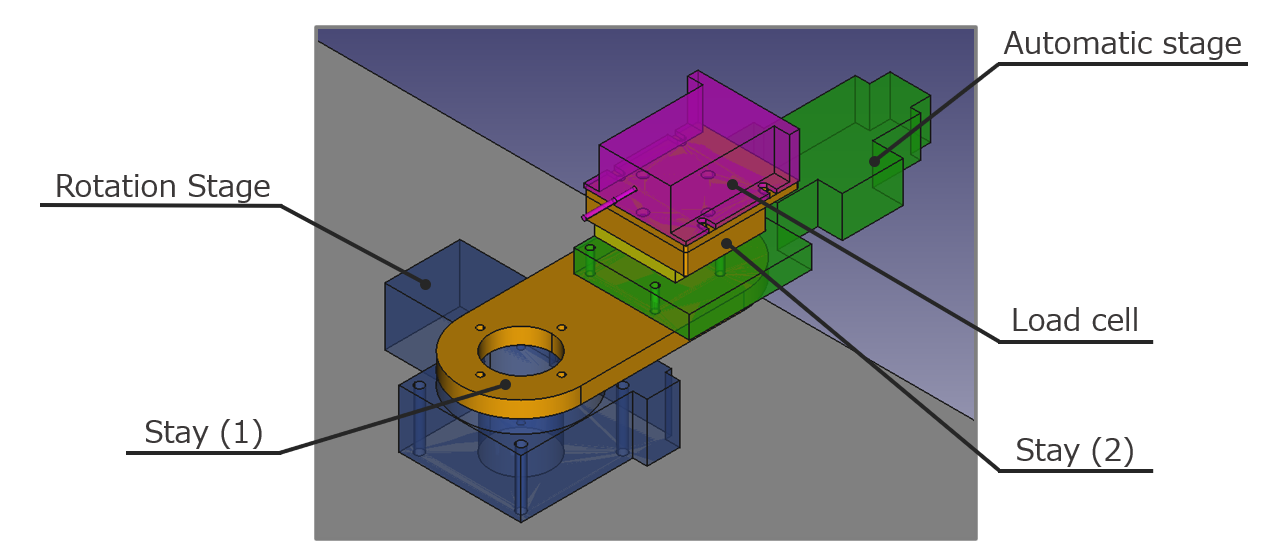
\includegraphics[width=120mm]{images/21-1.png}
        \caption{}
    \end{center}
\end{figure}

また,作用力測定装置のひずみセンサ,校正実験装置に取り付けられたロードセルからの出力電圧は
ストレインアンプを通して,ロガーへと送られ,ロガーに接続されたPCへと保存される.